\section{Experiments} \label{sec:experiments}
In this section, we put our proposed extension to practice. Specifically, we use the log-normal and exponentional components to approximate mixtures of Beta distributions. The log-normal and exponential components are selected because they have the same support on non-negative real values, and both have their respective inverse CDF functions available in closed-form. From \cref{fig:extension.single,fig:extension.multiple}, we see that in this particular setting, having two competing distribution families do not lead to significantly better approximations of the posterior. We now provide some analysis on what might have caused this.\\\\
In \cref{fig:extension.single}, standard ADVI's are run to approximate the Beta$(1,5)$ target using an exponential distribution and using a log-normal distribution. We see that both approximations approximates the target roughly equally well. In fact, the log-normal approximation seems to capture the tail a little bit better. However, note that both approximations fail to capture the increasing trend as the input approaches zero. This is not surprising given the shape of the log-normal distribution. However, it might have been unexpected to see the exponential distribution also failing to capture this shape, especially given that the target has a very similar shape to the exponential distribution. It is believed that this is likely due to the mapping used to convert the support of the exponential distribution from $(0,\infty)$ to $(0,1)$. Specifically, to map $(0,\infty)$ to $(0,1)$, the transformation $T_0(t) = \frac{1}{t+1}$ is used. As a result, the higher density region where the input is close to zero actually gets mapped to values that are among the smallest. This dip close to zero is clearly reflected in \cref{fig:extension.single}.\\\\
Similarly in \cref{fig:extension.multiple}, when approximating $0.5\text{Beta}(1,6) + 0.5\text{Beta}(30,10)$ using both types of components and only log-normal components, the two methods yield similar results. Again, using only log-normal components seem to approimxate the target distribution a little bit better. While the exponential component somewhat captures the upward trend as $x$ approaches zero, the quality of this approximation is hindered by the transformation $T_0$.

\begin{figure}[H]
\centering
\begin{subfigure}{0.45\textwidth}
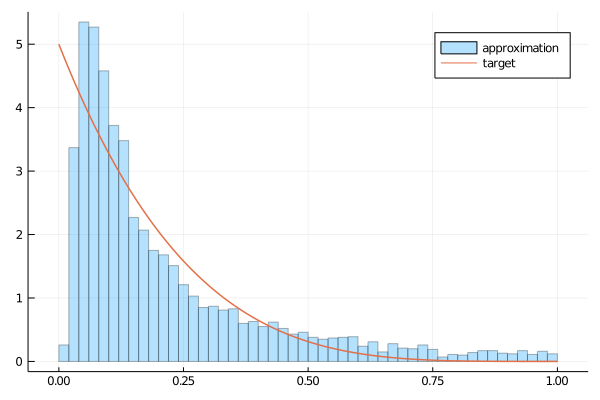
\includegraphics[width=1\linewidth]{../../plot/exp_single.png}
\caption{Approximating Beta$(1,5)$ using a single exponential component}
\end{subfigure}
\begin{subfigure}{0.45\textwidth}
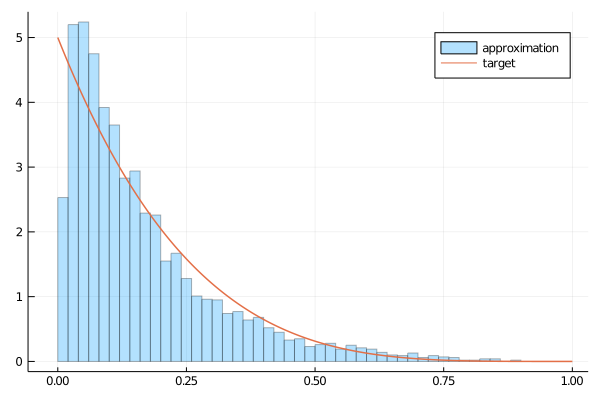
\includegraphics[width=1\linewidth]{../../plot/gauss_single.png}
\caption{Approximating Beta$(1,5)$ using a single log-normal component}
\end{subfigure}
\caption{Comparing the single component approximations on a Beta distribution.}
\label{fig:extension.single}
\end{figure}

\begin{figure}[H]
\centering
\begin{subfigure}{0.45\textwidth}
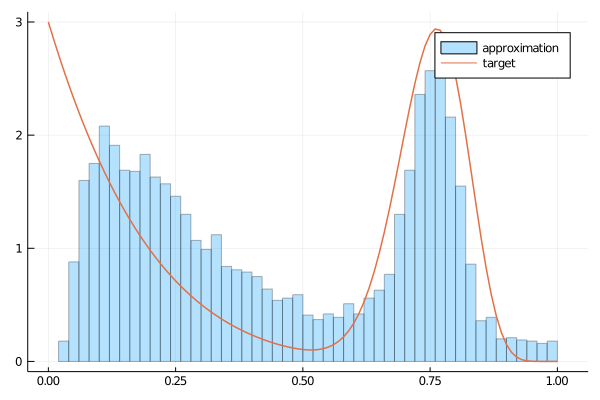
\includegraphics[width=1\linewidth]{../../plot/both_multiple.png}
\caption{Approximating a mixture of two Beta distributions using both an exponential and a log-normal component}
\end{subfigure}
\begin{subfigure}{0.45\textwidth}
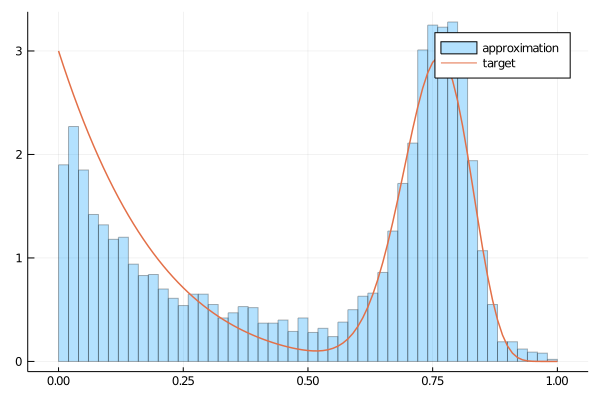
\includegraphics[width=1\linewidth]{../../plot/gauss_multiple.png}
\caption{Approximating a mixture of two Beta distributions using two log-normal components}
\end{subfigure}
\caption{Comparing the two-component approximations on a Beta mixture distribution.}
\label{fig:extension.multiple}
\end{figure}